\section{Geometric transfers to infinite and thermal paths}
\label{R:alt:g:section}

Finite bridge moments and planar avoidance give another route to the infinite-path
and thermal exponents. For the infinite path, a future renewal supplies
a useful averaging device. For the thermal path, inserting a tall bridge
separates the endpoints; the main issue is to control how many insertions
can produce the same walk. We give the two transfers together because they
use the same strip geometry, but their probability normalizations remain
separate.

We use the port convention of Proposition~\ref{R:renew:factorization}.
For a strict bridge $\eta$, $L(\eta)$ counts visited vertices and its weight
is $\rho^{L(\eta)}$. Set $B_0=1$ and let $B_h$ be the total weight of
bridges of height $h\ge1$ from a fixed bottom port, with the terminal
port free. Write $\beta=3/4$. The finite inputs are
\begin{align}
 B_h&\asymp(1+h)^{\beta-1},\label{R:alt:g:strip}\\
 F_h:=\sum_{\eta:\,H(\eta)=h}\rho^{L(\eta)}L(\eta)
   &\le h^{13/12+o(1)},\label{R:alt:g:first}\\
 \sum_{\substack{\eta:\,H(\eta)=h\\
                 \operatorname{lat}(\eta)>M}}
       \rho^{L(\eta)}&\le ChM^{-5/4}\qquad(M\ge C_1h).
       \label{R:alt:g:localization}
\end{align}
Here $\operatorname{lat}$ is the maximal horizontal distance from the
source, up to an immaterial fixed change of lattice coordinates.
The first estimate is \cite[Theorem~1.1]{Strip2026}; the second
is \cite[Proposition~11.5]{Nesting2026}. The third
is \cite[Lemma~4.1]{Geometry2026}. The first-length mass in \eqref{R:alt:g:first} is unnormalized: no division by $B_h$ has been made.

We also use three geometric results from \cite{Geometry2026}.
Lemma~5.1 there says that a critical renewal path, stopped at its
first renewal above height $h$, contains at least $h^{4/3-\xi}$ vertices
with probability $h^{-o(1)}$, for each fixed $\xi>0$. Proposition~3.1 there gives constants $C_0,C_1$ such that the
critical mass of all vertex walks confined to a box of side $R$, from
any specified vertex and with arbitrary endpoint and length, is at most
$C_0(1+R)^{C_1}$. Finally, let $S_2(r)$ be the probability that two independent renewal
paths from adjacent ports are disjoint through their respective first
visits to height $r$. Corollary~6.6 there gives
\begin{equation}\label{R:alt:g:avoidance}
 S_2(r)\le C_\varepsilon r^{-\beta+\varepsilon}
\end{equation}
for every $\varepsilon>0$. These statements use critical weights and the renewal probability law;
no thermal or uniform-length law is involved.

\subsection{Averaging over future renewals}

Let $S_0=0$ and $S_k=H_1+\cdots+H_k$ be the renewal heights under the
iid irreducible law $p$, and put
\[
 \tau_h=\min\{k:S_k>h\},\qquad
 \Gamma_h=\eta_1\circ\cdots\circ\eta_{\tau_h}.
\]
The last block can overshoot $h$. In particular, estimates for bridges
conditioned to end exactly at $h$ cannot be substituted directly for
estimates of $\Gamma_h$.

\begin{proposition}[Stopped renewal paths]\label{R:alt:g:infinite}
For every $\varepsilon>0$ there is $c_\varepsilon>0$ such that
\[
 \mathbb P\{h^{4/3-\varepsilon}\le L(\Gamma_h)
            \le h^{4/3+\varepsilon},\quad
             \operatorname{diam}(\Gamma_h)\le Ch^{1+\varepsilon}\}
       \ge1-O_\varepsilon(h^{-c_\varepsilon}).
\]
Consequently, if $\omega_n$ is the $n$-th vertex of the infinite
concatenation and its initial port is $o$, then almost surely
\[
 |\omega_n-o|=n^{3/4+o(1)},\qquad
 \#\{n:|\omega_n-o|\le R\}=R^{4/3+o(1)}.
\]
\end{proposition}
\begin{proof}
The factorization in Proposition~\ref{R:renew:factorization} gives
$\mathbb P\{m\text{ is a renewal height}\}=B_m$. If $I_j$ is the
probability that one irreducible has height $j$, the same factorization
and \eqref{R:alt:g:strip} give
\[
 \sum_{j\ge x}I_j\le Cx^{-\beta}.
\]
Indeed, $\sum_m B_me^{-m/x}\asymp x^\beta$, its reciprocal is
$1-\sum_j I_je^{-j/x}$, and this deficit bounds
$(1-e^{-1})\sum_{j\ge x}I_j$ from below. Decomposing according to the
last renewal before $h$, for $x\ge2h$ we obtain
\begin{equation}\label{R:alt:g:overshoot}
 \mathbb P\{S_{\tau_h}>x\}
   =\sum_{i=0}^{\lfloor h\rfloor} B_i
                        \sum_{j>x-i}I_j
   \le C(h/x)^\beta.
\end{equation}

For the length lower bound choose small $\theta,\xi>0$ and set
$a=\lfloor h^{1-\theta}\rfloor$,
$b=\lfloor h^{1-\theta/2}\rfloor$,
$k=\lfloor h^{\theta/16}\rfloor$. Run $k$ successive trials of
height $a$, restarting at each terminal renewal. They are independent
by the iid law after stopping renewal indices. If their height advances
are $\Delta_1,\ldots,\Delta_k$, then
\[
 \mathbb P\Big\{\sum_{i=1}^k\Delta_i>b\Big\}
 \le Ck(ak/b)^\beta\le Ch^{-17\theta/64}.
\]
The renewal-trial lemma gives success probability at least
$h^{-\theta/32}$ for each trial when $h$ is large. The probability
that all fail is at most $\exp(-c h^{\theta/32})$. Outside these two
exceptional events a trial of length at least $a^{4/3-\xi}$ is contained
in $\Gamma_b$, hence in $\Gamma_h$. Choose $\theta,\xi$ so that
$(1-\theta)(4/3-\xi)>4/3-\varepsilon$. This proves the required
polynomial lower-tail estimate.

For the upper bounds put $s=\lfloor h^{1+\delta}\rfloor$, where
$\delta>0$ will be small, and let $u=S_{\tau_h}$. The exceptional
probability $\mathbb P\{u>s\}$ is at most $Ch^{-\beta\delta}$.
Starting from $u$, the expected number of continuation renewals in the
next $s$ bands, including the renewal at $u$, is
\[
 D_s=\sum_{j=0}^sB_j\asymp s^\beta.
\]
Conditionally on $\Gamma_h$, this future renewal count has expectation
$D_s$. On $u\le s$ every such continuation ends at a height at most
$2s$ and contains $\Gamma_h$. Therefore
\begin{align*}
 D_s\,\mathbb E[L(\Gamma_h)\mathbf1_{\{u\le s\}}]
 &\le\sum_{m\le2s}
       \sum_{\eta:\,H(\eta)=m}\rho^{L(\eta)}L(\eta)\\
 &\le s^{25/12+o(1)}.
\end{align*}
The first inequality counts a subset of all renewal prefixes ending at
heights at most $2s$. Their distribution is the unnormalized bridge
measure, by the pathwise factorization; it does not require independence
between the length and the height of one irreducible. Markov's inequality
now gives
\[
 \mathbb P\{L(\Gamma_h)>h^{4/3+\varepsilon},\ u\le s\}
 \le h^{4\delta/3-\varepsilon+o(1)}.
\]

The same device controls horizontal excursions. If $\Gamma_h$ reaches
horizontal distance $M=h^{1+\varepsilon}$, all its continuation
prefixes do so. For $\delta<\varepsilon$, summing
\eqref{R:alt:g:localization} over their possible heights gives
\[
 D_s\,\mathbb P\{\operatorname{lat}(\Gamma_h)>M,\ u\le s\}
 \le C\sum_{m\le2s}mM^{-5/4}\le Cs^2M^{-5/4}.
\]
After division by $D_s$, this is at most
$Ch^{-5(\varepsilon-\delta)/4}$. On $u\le s$ the vertical span is
at most a fixed multiple of $s$. Taking $\delta=\varepsilon/4$,
with a smaller slack first if necessary, proves the assertion.

Apply Borel--Cantelli on dyadic values of $h$, simultaneously for a
countable sequence of positive slacks tending to zero. For each fixed
small $\eta>0$, eventually
\[
 h^{4/3-\eta}\le L(\Gamma_h)\le h^{4/3+\eta},\qquad
 \operatorname{diam}(\Gamma_h)\le Ch^{1+\eta}
\]
at every dyadic scale. A dyadic $h$ a fixed factor below
$n^{1/(4/3+\eta)}$ has $L(\Gamma_h)<n$; every subsequent vertex lies
above its terminal renewal line, whose height exceeds $h$. A dyadic
$h$ a fixed factor above $n^{1/(4/3-\eta)}$ has
$L(\Gamma_h)>n$. Hence, eventually,
\[
 c_\eta n^{1/(4/3+\eta)}\le|\omega_n-o|
 \le C_\eta n^{(1+\eta)/(4/3-\eta)}.
\]
Let $\eta\downarrow0$. The resulting pointwise bounds also show that
all sufficiently early indices, up to $R^{4/3-o(1)}$, are in the ball,
and all sufficiently late indices, beyond $R^{4/3+o(1)}$, are outside.
This proves the visit-count assertion.
\end{proof}

The fugacity interpretation of this same infinite law is supplied by
Lemma~\ref{R:renew:halfplane}. For $0<x<\rho$, let
$Z_{\mathrm{hp}}(x)$ be the normalizer of nonempty port-to-vertex
half-plane walks with weight $x$ per visited vertex. To check the
conventions here, a specified tuple of $j$ irreducibles of total vertex length $\ell$
followed by a nonempty path above its last seam has unnormalized mass
$x^\ell Z_{\mathrm{hp}}(x)$. Its probability is exactly $x^\ell$.
The tuple events are disjoint and their probabilities sum to
$J(x)^j$, where $J(x)=\sum_\eta x^{L(\eta)}\uparrow1$ as
$x\uparrow\rho$. Thus the complement has probability tending to zero
and the tuple weights tend to their critical values. Taking $j\ge m$
determines the first $m$ visited vertices and proves local convergence,
including vanishing probability of termination before the $m$-th vertex.
No uniform finite-length local limit is used in this argument.

\subsection{Tall-bridge insertions and their multiplicities}

We now work with ordinary walks rooted at a fixed vertex $o$, and write
$\ell(\gamma)$ for their number of edges. An insertion separates the two
arms of a walk by a bridge of height in $[H,2H]$ and diameter at most
$C_*H$, where $C_*$ is fixed. Its added mass will be of order $H^\beta$.
To use that mass, we must bound the number of inputs producing one output.

Split the input at its first lowest vertex. At an upward-pointing minimum,
extend both arms to the horizontal port immediately below it. A
downward-pointing minimum must be an endpoint, because an internal vertex
of that type cannot have both incident path edges above it. In that case
extend through the adjacent lower triangle and then to its bottom port.
Every added vertex lies below the original minimum and is therefore
unvisited. Reflect the backward arm below this common starting line,
insert the bridge, and place the forward arm above its upper line. The
three portions occupy disjoint open height layers, as in
Figure~\ref{R:alt:g:insertion-figure}.

The reflection interchanges the two honeycomb vertex types. Fix an output
root $o^*$ of the reflected type and translate the output so that the
reflected original root is $o^*$. Walk partition sums at $o$ and $o^*$ are
equal by a lattice reflection and translation. That symmetry preserves
edge length, diameter, and absolute endpoint-height difference.

Cutting the output at the two joining levels recovers the input and
inserted bridge up to a bounded local record. The port cuts subdivide
edges into half-edges; ports carry no vertex weight. Thus the output
edge weight differs from the product of the input edge weight and bridge
vertex weight by a bounded factor, uniformly for activities in
$[\rho/e,\rho]$. For a class $\mathcal A$ of input walks, let
$M_{\mathcal A}(\omega)$ count the insertion representations of an output
$\omega$ with input in $\mathcal A$. Each pair of joining levels determines
at most a fixed number of representations, independently of $h,H$.

\begin{figure}[ht]
\centering
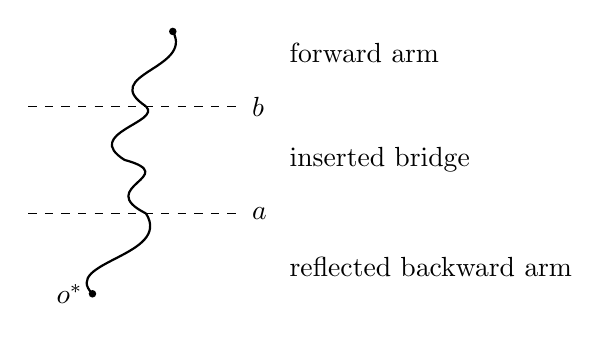
\begin{tikzpicture}[scale=.68]
 \draw[dashed] (-2,2)--(2,2) node[right] {$a$};
 \draw[dashed] (-2,4)--(2,4) node[right] {$b$};
 \draw[thick] (-.8,.5) .. controls (-1.4,1.1) and (.7,1.2) .. (.2,2);
 \draw[thick] (.2,2) .. controls (-.8,2.5) and (.9,2.7) .. (-.2,3)
             .. controls (-1,3.5) and (.5,3.7) .. (.2,4);
 \draw[thick] (.2,4) .. controls (-.7,4.6) and (1.1,4.7) .. (.7,5.4);
 \fill (-.8,.5) circle (2pt) node[left] {$o^*$};
 \fill (.7,5.4) circle (2pt);
 \node[anchor=west] at (2.7,1) {reflected backward arm};
 \node[anchor=west] at (2.7,3) {inserted bridge};
 \node[anchor=west] at (2.7,5) {forward arm};
\end{tikzpicture}
\caption{One insertion, with joining levels $a<b$. Cutting at these
levels and undoing the lower reflection recovers the input up to a
bounded local record. The drawing suppresses the modifications at the
ports.}
\label{R:alt:g:insertion-figure}
\end{figure}

\begin{lemma}[Insertion multiplicities]\label{R:alt:g:multiplicity}
Suppose $h\to\infty$ and $h/H\to0$. Let $\mathcal A_D$ be the walks
rooted at $o$ with diameter at most $h$. Every fixed integer $k\ge1$
satisfies
\begin{equation}\label{R:alt:g:diameter-moment}
 \sum_\omega\rho^{\ell(\omega)}M_{\mathcal A_D}(\omega)^k
       \le C_k H^{C+o_k(1)}h^{k\beta}.
\end{equation}
For fixed $K>0$, let $\mathcal A_E$ be the walks rooted at $o$ of length
at most $H^K$ and absolute vertical endpoint difference at most $h$.
Then
\begin{equation}\label{R:alt:g:endpoint-moment}
 \sum_\omega\rho^{\ell(\omega)}M_{\mathcal A_E}(\omega)^k
 \le C_{k,K}H^{C_K+o_k(1)}
             \{h^\beta(H/h)^{2\beta-1}\}^{k}.
\end{equation}
The sums run over outputs rooted at $o^*$. The exponents $C,C_K$ are
independent of $k$.
\end{lemma}
\begin{proof}
Write $M=M_{\mathcal A}$ for either input class and expand $M^k$ into
ordered $k$-tuples of representations of the same output. We first
locate their seams. Let $z_0,z_f$ be the vertical coordinates of the
output endpoints. Undoing the lower reflection sends the root to height
$2a-z_0$, while removing the inserted height sends the other endpoint to
$z_f-(b-a)$, up to bounded local changes. The original endpoint difference
is therefore $z_0+z_f-a-b+O(1)$. Both input classes satisfy
\begin{equation}\label{R:alt:g:seam-sum}
 |a+b-z_0-z_f|\le C_2h,\qquad H\le b-a\le2H.
\end{equation}
All heights here are in row units, with fixed conversion factors absorbed
in $C_2$.

Put $S=z_0+z_f$ and $E=C_2h$. The possible seams lie in the intervals
\[
 a\in\left[\frac{S-E-2H}{2},\frac{S+E-H}{2}\right],\qquad
 b\in\left[\frac{S-E+H}{2},\frac{S+E+2H}{2}\right].
\]
Every upper seam thus exceeds every lower seam by at least $H-E>0$
for large $H$. Sort the lower seams increasingly and the upper seams
decreasingly:
\[
 a_1\le\cdots\le a_k<b_k\le\cdots\le b_1.
\]
Record ties and the original representation pairing by a permutation
$\pi$: the representation with lower seam $a_i$ has upper seam
$b_{\pi(i)}$. These records cost a factor depending only on $k$.

Every positive gap between consecutive seams in either group is a strict
bridge. The two exterior portions and the portion between $a_k$ and $b_k$
are the only three portions left over. In the diameter case the whole
output lies in a box of side $O(H)$; in the endpoint case it lies in a box
of side $O(H+H^K)$. Fixing the output endpoint and the four extreme seam
ports costs a polynomial in $H$ whose exponent is independent of $k$.
The full-box susceptibility bound then sums the three leftover portions
at cost $H^C$ or $H^{C_K}$. Internal joining ports introduce no additional
position sums: once the relative gap shapes are specified, each has a
unique translation to its joining port.

For the remaining gaps, use heights
\[
 s_1=t_1=0,\qquad
 s_i=a_i-a_{i-1},\quad t_i=b_{i-1}-b_i\quad(2\le i\le k).
\]
The zero slots account for the two extreme seams. Repeated seams give
further zero gaps, with bounded weight. The lower gap of height $s_i$
ends at $a_i$, and the upper gap of height $t_j$ starts at $b_j$.
Consequently the original representation $i$ pairs the slots
$(s_i,t_{\pi(i)})$. Every positive gap appears in exactly one such pair.
Figure~\ref{R:alt:g:pairings-figure} distinguishes this pairing from the
rank pairing used later to sum endpoint constraints.

\begin{figure}[ht]
\centering
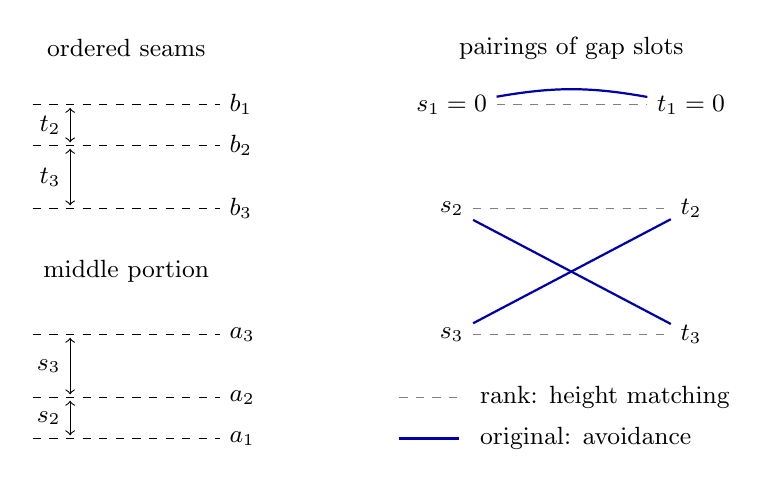
\begin{tikzpicture}[x=.95cm,y=.8cm,font=\small]
 \node at (1.25,6.2) {ordered seams};
 \draw[dashed] (0,0)--(2.5,0) node[right] {$a_1$};
 \draw[dashed] (0,.65)--(2.5,.65) node[right] {$a_2$};
 \draw[dashed] (0,1.65)--(2.5,1.65) node[right] {$a_3$};
 \draw[dashed] (0,3.65)--(2.5,3.65) node[right] {$b_3$};
 \draw[dashed] (0,4.65)--(2.5,4.65) node[right] {$b_2$};
 \draw[dashed] (0,5.3)--(2.5,5.3) node[right] {$b_1$};
 \draw[<->] (.5,.05)--(.5,.60) node[midway,left] {$s_2$};
 \draw[<->] (.5,.70)--(.5,1.60) node[midway,left] {$s_3$};
 \draw[<->] (.5,3.70)--(.5,4.60) node[midway,left] {$t_3$};
 \draw[<->] (.5,4.70)--(.5,5.25) node[midway,left] {$t_2$};
 \node at (1.25,2.65) {middle portion};
 \node at (7.2,6.2) {pairings of gap slots};
 \node (s1) at (5.6,5.3) {$s_1=0$};
 \node (s2) at (5.6,3.65) {$s_2$};
 \node (s3) at (5.6,1.65) {$s_3$};
 \node (t1) at (8.8,5.3) {$t_1=0$};
 \node (t2) at (8.8,3.65) {$t_2$};
 \node (t3) at (8.8,1.65) {$t_3$};
 \draw[dashed,gray] (s1)--(t1);
 \draw[dashed,gray] (s2)--(t2);
 \draw[dashed,gray] (s3)--(t3);
 \draw[thick,blue!65!black] (s1) to[bend left=10] (t1);
 \draw[thick,blue!65!black] (s2)--(t3);
 \draw[thick,blue!65!black] (s3)--(t2);
 \draw[dashed,gray] (4.9,.65)--(5.7,.65);
 \node[anchor=west] at (5.85,.65) {rank: height matching};
 \draw[thick,blue!65!black] (4.9,0)--(5.7,0);
 \node[anchor=west] at (5.85,0) {original: avoidance};
\end{tikzpicture}
\caption{Three representations of one output. The left panel shows the
seam order and the positive gaps; the two extreme slots have height zero.
The right panel illustrates the original permutation
$\pi(1)=1$, $\pi(2)=3$, $\pi(3)=2$. Rank pairs constrain the two gap
heights; original pairs inherit avoidance from an input walk. Connecting
lines in the right panel match variables and do not represent walk
segments. The diagram is not to scale.}
\label{R:alt:g:pairings-figure}
\end{figure}

\paragraph{The diameter class.}
All its gap heights are $O(h)$: each lower seam is within $O(h)$ of
the root height, and each upper seam is within $O(h)$ of the final
height. Put the two gap heights in an original pair into dyadic bins
of scales $\sigma,\tau\le Ch$, with scale one for absent or bounded
gaps. The total bridge mass in a bin of scale $\sigma$ is at most
$C\sigma^\beta$, by \eqref{R:alt:g:strip}.

For two large gaps in an original pair, reverse and reflect the lower
one from its upper endpoint. The two resulting pieces are initial
portions of the input arms at its minimum and avoid one another after
their common first vertex. Move one start to the adjacent port and pass
through the neighboring upward triangle to the same first upper
neighbor. If that triangle was already visited, strictness at the lower
wall forces the visit immediately after the first upper neighbor;
start there and delete the short initial segment. The other arm cannot
use that triangle because it would also use the same upper neighbor.
This recoding has bounded inverse ambiguity and preserves avoidance
through first visits to height $q=c\min(\sigma,\tau)$, for a fixed small
$c>0$. Thus it gives the adjacent-port event in
\eqref{R:alt:g:avoidance}.

Expose each gap from its assigned end through its first renewal at or
above $q$. If the exposed height is $u$, the remaining critical mass
at terminal height $v$ is $B_{v-u}$, with $B_j=0$ for $j<0$. Uniformly
in the exposed shape,
\[
 \sum_{v\le C\sigma}B_{v-u}\le C\sigma^\beta.
\]
The exposed strings have the independent renewal probability law.
After integrating the completions, the paired integral is therefore at
most
\[
 C\sigma^\beta\tau^\beta\min(\sigma,\tau)^{-\beta}H^{o(1)}
 =C\max(\sigma,\tau)^\beta H^{o(1)}
 \le Ch^\beta H^{o(1)}.
\]
If one gap is absent or bounded, the ordinary mass bound for the other
proves the same estimate. Normalize every gap at its assigned test end
and drop all other intersection restrictions. The pairs
$(s_i,t_{\pi(i)})$ use disjoint gap variables, so their bounds multiply
by Tonelli's theorem. The $(1+\log H)^{O(k)}$ dyadic choices contribute
$H^{o_k(1)}$. Together with the three leftover portions, this proves
\eqref{R:alt:g:diameter-moment}.

\paragraph{The endpoint class.}
Its gaps can have height of order $H$, but their rank pairing retains a
constraint. The original pairs satisfy
$|a_i+b_{\pi(i)}-S|\le E$. Two ordered multisets admitting a matching
within $E$ also admit the monotone matching within $E$. Applied to
$a_i$ and $S-b_j$, this gives
\[
 |a_i+b_i-S|\le E,\qquad |s_i-t_i|\le2E\quad(2\le i\le k).
\]
We use these rank pairs to integrate the completion heights, while
keeping $\pi$ for the subsequent avoidance tests.

For a gap in a dyadic bin of scale $\sigma$, put
$w_\sigma=\min(h,\sigma)$ and expose its renewal string through height
$c w_\sigma$, using threshold zero for a bounded gap. Condition on
all exposed strings. A rank pair with one height $O(h)$ has both
heights $O(h)$ and completion mass at most
$Cw_\sigma^\beta w_\tau^\beta$. For a rank pair at comparable scales
$r,r'\gg h$, uniformly in the exposed heights $u_0,v_0$, the completion
mass is at most
\begin{align*}
 &\sum_{\substack{u\asymp r,\ v\asymp r'\\
                |u-v|\le2E,\ u\ge u_0,\ v\ge v_0}}
         B_{u-u_0}B_{v-v_0}\\
 &\hspace{15mm}\le Chr^{2\beta-1}
 \le Cw_r^\beta w_{r'}^\beta(H/h)^{2\beta-1}.
\end{align*}
For the first inequality fix $u-v$, apply Cauchy--Schwarz to the two
translated sequences, and use
$\sum_{j\le Cr}B_j^2\le Cr^{2\beta-1}$; there are $O(h)$ allowed
differences. Here $2\beta-1=1/2>0$. An exposed string that overshoots
its possible endpoint contributes zero, so the bound is uniform without
an extra overshoot condition.

Integrating all completion variables by rank pairs leaves one factor
$w_\sigma^\beta$ per gap and at most $k$ factors
$(H/h)^{2\beta-1}$. The remaining measure is the product of the
independent stopped-string laws. Regroup them now by their original
pairs $(s_i,t_{\pi(i)})$. Each avoidance test costs
$\min(w_\sigma,w_\tau)^{-\beta}H^{o(1)}$, and hence each original
pair contributes at most
\[
 w_\sigma^\beta w_\tau^\beta
       \min(w_\sigma,w_\tau)^{-\beta}H^{o(1)}
 \le h^\beta H^{o(1)}.
\]
Every string is used once. Multiplying these bounds, summing the dyadic
bins, and restoring the polynomial cost of the three leftover portions
proves \eqref{R:alt:g:endpoint-moment}.
\end{proof}

\subsection{The thermal deduction}

Let $c_m$ count unrestricted $m$-edge walks from a fixed vertex, including
the empty walk, and for $T>1$ set
\[
 x_T=\rho e^{-1/T},\qquad
 Z_T=\sum_{m\ge0}c_mx_T^m,\qquad
 \mathbb P_T^{\mathrm{th}}(\gamma)=Z_T^{-1}x_T^{\ell(\gamma)}.
\]
We also use the diameter clause of \cite[Theorem~1.1]{Geometry2026}:
for every $\eta>0$, every finite $A>0$ and every integer $m\ge1$,
the uniform law on $m$-edge walks satisfies
\begin{equation}\label{R:alt:g:uniform-upper}
 \mathbb P_m\{\operatorname{diam}(\gamma)>m^{3/4+\eta}\}
       \le C_{\eta,A}m^{-A}.
\end{equation}
This is an all-length upper bound; the thermal deduction does not
require an all-length uniform endpoint lower bound.

\begin{proposition}[Thermal stretching by insertion]
\label{R:alt:g:thermal}
Under $\mathbb P_T^{\mathrm{th}}$, as $T\to\infty$,
\[
 \begin{gathered}
 \ell(\gamma)=T^{1+o(1)},\qquad
 \operatorname{diam}(\gamma)=T^{3/4+o(1)},\\
 |\gamma_{\ell(\gamma)}-\gamma_0|=T^{3/4+o(1)}
 \end{gathered}
\]
in probability. Each statement means convergence within every fixed
positive exponent slack.
\end{proposition}
\begin{proof}
Every $m$-edge walk lies in a box of side $O(m)$, so full-box
susceptibility gives $c_m\rho^m\le C(1+m)^C$. In particular $Z_T$ is
finite, $Z_T\ge1$, and for every $\xi>0$,
\begin{equation}\label{R:alt:g:thermal-length-upper}
 \mathbb P_T^{\mathrm{th}}\{\ell(\gamma)>T^{1+\xi}\}
 \le\sum_{m>T^{1+\xi}}C(1+m)^Ce^{-m/T}=o(1).
\end{equation}
We first prove the endpoint lower bound on lengths at most $T^2$.
This restriction loses $o(1)$ probability and permits use of the second
multiplicity estimate.

Fix a small $\zeta>0$ and set
$h=T^{3/4-\zeta}$, $H=T^{3/4-\zeta/2}$, rounding heights to integers.
The critical mass of bridges of height in $[H,2H]$ is comparable to
$H^\beta$. By \eqref{R:alt:g:localization}, choosing the fixed
confinement constant $C_*$ sufficiently large retains a fixed fraction
with diameter at most $C_*H$. The mass of bridges in this height window
with $L(\eta)>T$ is at most $T^{-1}H^{25/12+o(1)}$, by
\eqref{R:alt:g:first}. Its ratio to $H^\beta$ is
$H^{4/3+o(1)}/T=o(1)$. On the remainder,
$x_T^{L(\eta)}\ge e^{-1}\rho^{L(\eta)}$. Thus every input admits
insertions of total $x_T$-mass at least $cH^\beta$.

Let $\mathcal A$ consist of inputs of length at most $T^2$ whose absolute
vertical endpoint difference is at most $h$, and let $V$ be their
$x_T$-mass. Since $T^2\le H^K$ for a fixed sufficiently large $K$,
Lemma~\ref{R:alt:g:multiplicity} applies to $M_{\mathcal A}$. Put
\[
 A_h=h^\beta(H/h)^{2\beta-1}\le H^\beta,
 \qquad Q=A_hH^\delta,
\]
where $\delta>0$ will be chosen small after $\zeta$. For every fixed
integer $k\ge1$, the lemma gives
\begin{align*}
 \sum_{M_{\mathcal A}(\omega)>Q}
       x_T^{\ell(\omega)}M_{\mathcal A}(\omega)
 &\le Q^{1-k}\sum_\omega
       \rho^{\ell(\omega)}M_{\mathcal A}(\omega)^k\\
 &\le C_{k,K}A_hH^{C_K+o_k(1)-\delta(k-1)}.
\end{align*}
Choose $k$ so that $\delta(k-1)>C_K+\beta+1$, and then let
$T\to\infty$. The last expression is $o(1)$. This order is possible
because $C_K$ is independent of $k$.

Sum all insertions of inputs in $\mathcal A$. For outputs with
$M_{\mathcal A}\le Q$, there are at most $Q$ representations per
output. Their unrestricted partition sum, rooted at $o^*$, equals
$Z_T$ by the root symmetry established above. The preceding estimate
handles the remaining outputs. Recoverability and the bounded weight
factors therefore give
\begin{equation}\label{R:alt:g:insertion-mass}
 cH^\beta V\le C A_hH^\delta Z_T+o(1).
\end{equation}
Divide by $H^\beta Z_T$ and use
\[
 \frac{A_h}{H^\beta}=(h/H)^{1-\beta}.
\]
For sufficiently small $\delta$, the bound
$V/Z_T\le C(h/H)^{1-\beta}H^\delta+o(1)$ tends to zero. Adding the
discarded length tail proves that the absolute vertical endpoint
difference exceeds $T^{3/4-\zeta}$ with probability tending to one.
The Euclidean endpoint distance has the same lower exponent after
absorbing the fixed row-spacing factor into the slack.

It remains to obtain the diameter upper bound and the length lower
bound. Conditioned on its length, the thermal law is uniform. Fix
$\varepsilon>0$ and choose $\eta,\xi>0$ so that
\[
 (1+\xi)(3/4+\eta)<3/4+\varepsilon.
\]
For $m<T^{1/2}$ the diameter is deterministically at most $CT^{1/2}$.
For $T^{1/2}\le m\le T^{1+\xi}$, the probability of violating
$D\le T^{3/4+\varepsilon}$ is, by
\eqref{R:alt:g:uniform-upper}, at most
$C_{\eta,A}T^{-A/2}$ under each conditional length law. The remaining
lengths have probability $o(1)$ by
\eqref{R:alt:g:thermal-length-upper}. This proves the upper diameter
exponent, and hence the upper endpoint exponent.

For the lower length bound it suffices to take $0<\xi<1/2$.
Choose $\eta,\zeta>0$ such that
\[
 (1-\xi)(3/4+\eta)<3/4-\zeta,
 \qquad \zeta<1/4.
\]
The typical endpoint lower bound excludes lengths $m<T^{1/2}$
deterministically. For $T^{1/2}\le m<T^{1-\xi}$, it forces
$D>m^{3/4+\eta}$, up to a fixed factor absorbed by the strict exponent
inequality. Equation~\eqref{R:alt:g:uniform-upper} bounds the conditional
probability of this event uniformly by $C_{\eta,A}T^{-A/2}=o(1)$.
Thus $\ell\ge T^{1-\xi}$ with probability tending to one. Together
with the length upper tail and $A\le D$, this proves all three claims.
\end{proof}
